%%% START A [ 443 words ]

\subsection{Motor Programs}

In this final technical section, we sketch out a possible solution to the problem of motion planning in order to illustrate how an engineer might go about utilizing research in neuroscience to solve a system-wide problem. While we don't directly discuss the problem of automated programming, it is exactly this problem in the context of the programmer's apprentice that motivates our interest in the problem of motion planning.

Our brains derive much of their utility from exploiting distributed representations and parallel processing. Even so, in big brains it is often useful bring representations from distant parts of the brain together and necessary to perform some computations serially with the results from one computation feeding into another. We have evolved machinery that makes it possible for us to do both by making better use of existing memory systems and adapting circuits optimized for movement in order to communicate, plan and perform abstract reasoning.

The mammalian brain makes extensive use of topographically organized representations, often contructing multiple maps with same topographic organization that can be aligned with one another to construct more abstract representations that retain the locality relationships of their constituent maps~\cite{WandelletalNEURON-07,WandelletalPTRS-B-05}. 

The basal ganglia have access to the sensorimotor areas of the cerebral cortex by way of the thalamus and the striatum, the latter being part of the basal ganglia. The thalamus consists of a set of nuclei that map specific subcortical inputs to the cortex and receive feedback from the same cortical areas. The striatum assists in coordinating cognitive functions, including both motor and action planning.

\begin{center}
  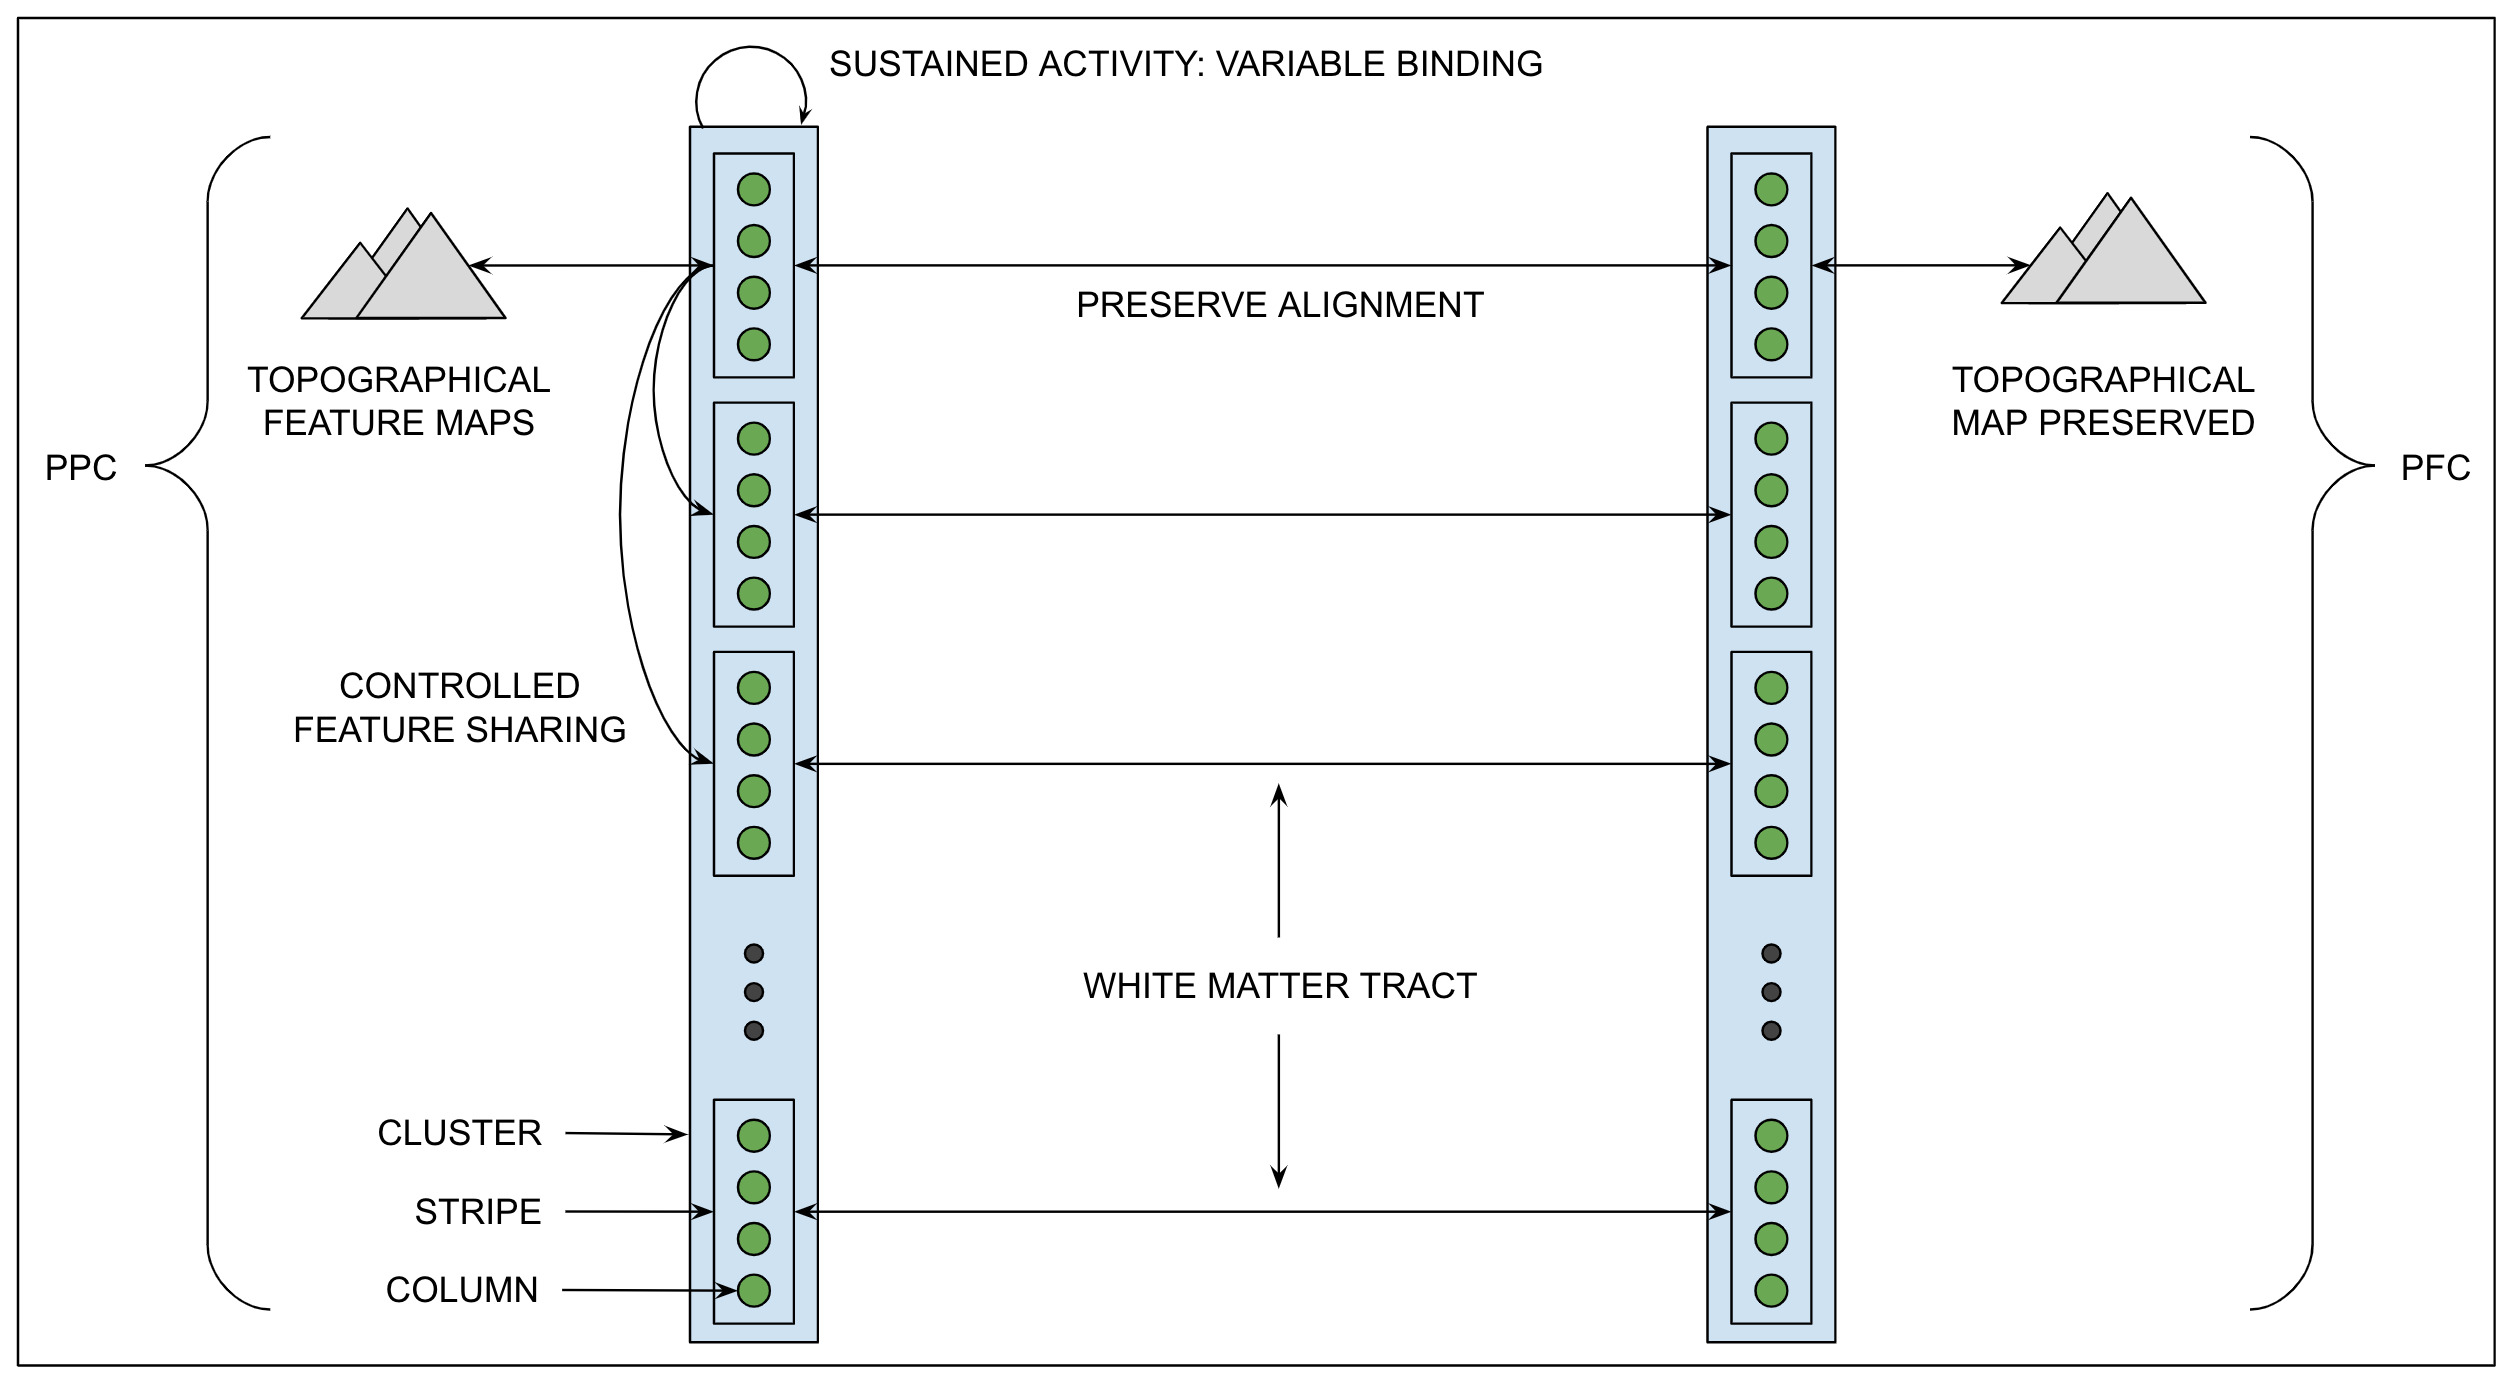
\includegraphics[width=200pt]{./figures/Columns_Stripes_Clusters_Topographic_Maps.jpg}
\end{center}

The striatum's distinctive striated appearance is due to its arrangement of specialized circuits called {\it{stripes}} that enable the basal ganglia to select and transfer information to other locations in the cortex that have similarly functioning circuits, preserving essential topographical features in the process~\cite{BarbasandGarcia-CabezasCOiN-16,LewisetalJNC-02}.

Each stripe is composed of columnar-shaped circuits called {\it{minicolumns}} that encode patterns of coordinated activity originating elsewhere in the cortex so it can brought together in one place for processing. These patterns of activity can be stored indefinitely providing a working memory system that supports a simple yet powerful method for binding variables and composing their values~\cite{OReillyetalCCN-12}.

Stripes are grouped in {\it{clusters}} that map to other clusters often by way of white-matter tracts that connect distant sensory and motor areas. Information is transferred preserving its topographic structure so processed information resulting from motion planning or other cognitive functions can be mapped back to its origin to support learning.

%%% STOP A 
%%% START B [ 678 words ] 

In robot motion planning, the degrees of freedom determined by a robot's effectors define a vector space called the {\it{configuration space}} of the physical system and the reachable space accounting for nearby obstacles and mechanical limitations is a lower-dimensional manifold called the {\it{configuration manifold}}. Any possible movement the robot can make corresponds to path on the configuration manifold.

The above characterization of robot motion planning doesn't account for the role of perception and feedback. Robust motion plans must necessarily include perceptual activities whose purpose it is to help guide movement, avoid obstacles including one's own body parts and facilitate accurate positioning and grasping.      

To serve as a basis for motion planning, an internal representation must capture not only the physical constraints that the body and environment impose on movement, but also the cognitive state of the agent incorporating current estimates of the location and velocity of nearby objects and body parts relative to the body's frame of reference and relevant knowledge about their properties and role in the agent's objectives.

Motor plans are represented in the primary, premotor and supplementary motor cortex in the frontal cortex adjacent to the central sulcus. The nearby somatosensory and proprioceptive association areas of the anterior parietal cortex are likely to figure prominently in planning movement, as are the sensory association areas in the posterior parietal cortex and in particular the dorsal visual stream also known as the "where" or "how" stream. These sources of relevant neural activity provide the basal ganglia with a rich context for guiding action selection.

We know that regions of the motor cortex are topographically organized, effectively combining information from sensorimotor areas throughout cortex to create a composite map or {\it{augmented configuration manifold}} for planning purposes. In lieu of an internal representation for abstract goals, we borrow the term {\it{setpoint}} from control theory to denote the target state provided by basal ganglia. Negative feedback systems use the difference between the system state and the setpoint to guide action selection and are common in biological organisms~\cite{Ashby1957cybernetics}.

The complete context for acting is a composite summary of the agent's sensorimotor, proprioceptive and vestibular state derived from a hierarchy of primary, secondary and associative features that constitute an abstraction hierarchy~\cite{FusterPREFRONTAL-CORTEX-15-CHAPTER_8} and roughly aligns with the features available to the basal ganglia and prefrontal cortex for modulating action selection.

The division of labor between the basal ganglia, motor cortex and cerebellar cortex is pretty well established. The basal ganglia do not directly select motor programs but rather they enable them to run in the motor cortex. The motor cortex selects and executes motor programs issuing motor commands via the descending pathways. The cerebellum does not initiate motor commands but rather modifies the motor commands of the descending pathways to make movements more adaptive and accurate. 

In the model for motor control presented here, the basal ganglia initiate a motor program in the motor cortex by creating a context for action corresponding to a desired future state. Since the motor cortex already has access to this information, all that is required of the basal ganglia is an offset from the current context to serve as a setpoint, thereby enabling the motor cortex to select an appropriate motor program for generating motor commands. Execution then consists of repeatedly invoking the selected motor program to traverse the augmented configuration manifold from the current context to the specified offset / setpoint.

The actions available in the process of executing a motor program include motor commands in the form of muscle contraction and relaxation and sensorimotor activities in service to visual {\emdash{}} or other sensory modality {\emdash{}} servoing of the sort required for grasping objects and avoiding obstacles. Methods for path planning such as artificial potential field methods~\cite{KhatibIJRR-86} or strategies for sensor-based traversals with randomized recovery could easily be incorporated in this model~\cite{LiarokapisetalICAR-15}. As for learning how to carry out and coordinate more complicated movements and manipulations, decades of research developing models of the cerebellum offer practical suggestions.

%%% STOP B %%% START C [ 561 words ]

In the 1970's James Albus~\cite{AlbusMB-71}, Masao Ito~\cite{Ecclesetal1967neuronal} and David Marr~\cite{MarrJoP-69} developed a model of the mammalian cerebellum about the same time that David Marr was working on his model. The Marr-Albus-Ito theory {\emdash{}} is still the {\urlh{https://en.wikipedia.org/wiki/Cerebellum#Theories_and_computational_models}{foundation}} on which most theories of the cerebellum are built.

Albus went on to work in applied robotics~\cite{AlbusetalSME-84} and invented a new approach to robotic control~\cite{Albus75} that he christened the {\it{cerebellar model articulation controller}} ({\urlh{https://en.wikipedia.org/wiki/Cerebellar_model_articulation_controller}{CMAC}}) and that is widely used in reinforcement learning for classification and control problems. In context of the discussion here, The CMAC controller essentially works by associating points in control space with assignments to servomotors in joint space in the case of articulated assembly robots.

To recap, in the first stage, the basal ganglia propose a motor program specified as a setpoint offset from a suitably compressed version of the current state vector that you can think of as a goal or intention. In the second stage, circuits in the motor cortex implement a negative feedback controller to drive the system toward the target setpoint. To accomplish the goal of reaching the supplied setpoint, these circuits attempt to trace a path along the configuration manifold representing the set of reachable system states.

%%% define association cortex earlier in the Neuroscience section 

How has neuroscience informed this model of motion planning? [...] (a) activity throughout the association cortex can reconstituted in other locations for processing (b) an approach to variable binding and persistent actively maintained persistent working memory (c) convolutional layers that learn topographically organized feature maps that can be registered with one another and combined to create composite maps that serve as representations for planning (d) an approach to learning mappings from latent states to latent actions to serve decision making [...] namely, Fuster's hierarchy \emdash{} see Figure~{\urlh{#fig_Coupled_Sensory_Motor_Hierarchy}{\ref{fig_coupled}}} \emdash{} consisting of parallel stacks of levels, each level in each stack a multi-layer network with the motor network reciprocally connected with the corresponding sensory network and the hierarchy trained from bottom (most concrete) to top (most abstract) [...] 

\section{Discussion}

In this paper we set out to illustrate how neuroscience might accelerate progress on some of the most challenging problems facing the field of artificial intelligence. We looked at seemingly hard problems like consciousness that have relatively simple engineering solutions, and seemingly easy problems like motion planning the require the integration of multiple memory and control subsystems.

We didn't discuss in any detail the implementation of the programmer's apprentice, and yet every one of the architectural vignettes that we discussed was instigated by our goal to develop end-to-end solutions for concrete engineering problems like the apprentice. Neither did we address one of the most challenging problems facing AI in the coming decade, namely the problem of training complex of the models we described here.

In terms of training, we believe that research in comparative and developmental cognitive neuroscience will prove invaluable in seeking effective solutions for training the next generation of AI systems that aspire to human-level competence. Perhaps in our next paper we will lay out our plans to train systems like the apprentice that have to collaborate closely with humans in order to solve complex engineering problems. 

%%% Stop C